% ======================================================================
%  Kapitel: Die Synthese-Pipeline  --  gekuerzte Fassung
%
%  Vorausgesetzt werden die Makros \code, \absatz, \px, \Oe sowie
%  biblatex, booktabs, tabularx, tikz (mit arrows.meta), subcaption.
%
%  Angleichungen an die korrigierten Vorkapitel:
%    - A-Nummern nach der Liste in Kap. 3 (A1 Labelgenauigkeit,
%      A2 Objektgroessen, A3 Groessenabhaengigkeiten, A4 Signaturen,
%      A5 kontrollierbare Variation, A6 Trennung Annahme/Messung)
%    - \ref{sec:sim2real} setzt ein \label{sec:shortcut} an der
%      Shortcut-Learning-Stelle in Kapitel 3 voraus (dort noch ergaenzen)
%
%  Gegenueber der Vorfassung gekuerzt: Farbangleich, Rauschschaetzung,
%  Nachweisabschnitt (jetzt Tabelle), Bildunterschriften, Einstieg der
%  Sichtbarkeitsrechnung. Die deaktivierte Abbildung zur Rauschschaetzung
%  ist entfernt -- sie liegt separat unter paper/entwuerfe/.
%
%  Mit "% PRUEFEN" markierte Stellen enthalten Zahlen, die sich
%  gegenseitig widersprechen und die ich nicht aufloesen kann.
% ======================================================================

\chapter{Datengrundlage und Synthese-Pipeline}
\label{kap:pipeline}

Dieses Kapitel vermisst zunächst das verfügbare Quellmaterial und dokumentiert
anschließend die Pipeline, die daraus (aus neun Objektausschnitten und sieben
Hintergrundaufnahmen) den Trainingsdatensatz erzeugt;
Abbildung~\ref{abb:pipeline} zeigt Herkunft der Bausteine und Reihenfolge der
Stufen im Überblick. Die in Tabelle~\ref{tab:parameter} genannten Anteile sind
keine konfigurierten Sollwerte, sondern \emph{gemessene} Ist-Werte aus dem
Erzeugungsbericht \code{synth/train/generation\_report.json} über 6000 Bilder
mit 173\,100 gerenderten Instanzen und 136\,384 gelabelten Objekten.

% ======================================================================
%  Kapitel: Datengrundlage  --  korrigierte und gekuerzte Fassung
%
%  Kapitelfragment, keine eigene Praeambel. Vorausgesetzt werden die
%  bereits in der Arbeit definierten Makros und Umgebungen:
%    \code{...}     Monospace-Auszeichnung
%    \absatz{...}   Absatzueberschrift
%    \px            Pixel-Einheit
%    \Oe            Objektdurchmesser als Einheit
%    L{...}         linksbuendiger Spaltentyp fester Breite (array/tabularx)
%  sowie biblatex (\parencite) und die Pakete booktabs, tabularx.
%
%  Querverweise auf Kapitel 3 verwenden die Labels der korrigierten
%  Kapitelfassung: eq:deff (3.8), eq:gridmiss (3.11), eq:bendavid (3.12).
%  Der Verweis \ref{subsec:kleine-objekte} zeigt dort auf
%  \label{subsec:kleine-objekte} -- Labelnamen ggf. angleichen.
% ======================================================================

\chapter{Datengrundlage}
\label{kap:daten}

Alle Parameter der folgenden Kapitel berufen sich auf Messungen am verfügbaren
Quellmaterial. Dieses Kapitel dokumentiert sie. Sämtliche Zahlenwerte sind mit
\code{src/analyze\_data.py} an den Quelldateien gemessen und in
\code{docs/datensichtung.json} abgelegt.

\section{Annotationsdefinition}
\label{sec:annotation}

Vor jeder Messung steht die Frage, was ein Objekt ist. Aus der Sichtung der
beiden handannotierten Realbilder ergibt sich eine Definition, die die gesamte
Pipeline prägt:

\begin{quote}
Annotiert ist ausschließlich die \textbf{sichtbare Stirnfläche} eines
Rundrohrprofils -- heller verzinkter Kranz, dunkle Bohrung. Rohrschäfte in
Seitenansicht, Gitterknoten und dunkle Löcher im Maschendraht sind
\textbf{keine} Objekte, obwohl sie ähnlich aussehen. Die Box umschließt den
\textbf{sichtbaren} Teil (modale Box), nicht den geschätzten vollständigen Kreis.
\end{quote}

Beide Festlegungen sind folgenreich: Die erste bestimmt, welche Strukturen als
harte Negative benötigt werden, die zweite, wie die Boxen im Generator berechnet
werden. Die Unterscheidung modal / amodal ist in der Literatur etabliert
\parencite{li2016amodal,zhu2017amodal}; amodale Boxen umschließen auch verdeckte
Teile. Erzeugte der Generator amodale Boxen, während die Realbilder modal
annotiert sind, entstünde ein systematischer Größenversatz -- ein Verstoß gegen
Anforderung~A5.

\section{Quellmaterial}
\label{sec:quellmaterial}

\absatz{Objektausschnitte.} Verfügbar sind neun aus Realaufnahmen
ausgeschnittene Rohrprofile der Größe $28\times30$ bis $43\times38$ Pixel. Sechs
zeigen eine dunkle Bohrung (offenes Rohr), drei eine helle (Sonnenlicht fällt in
die Röhre oder das Ende ist gestaucht); beide Formen kommen in den Realbildern
vor, weshalb gleichverteilt aus allen neun gezogen wird. Die aus dem
Ellipsenmodell gewonnenen Achsverhältnisse der Ausschnitte streuen zwischen 0,83
und 1,14 (Abschnitt~\ref{sec:matting}). Kritisch ist Befund~1 in
Tabelle~\ref{tab:befunde}: Alle neun sind zwar RGBA-Dateien, ihr Alphakanal ist
aber durchgängig 255 -- es handelt sich um rechteckige Ausschnitte, bei denen
13--35\,\% der Fläche nicht zum Objekt gehören.

\absatz{Hintergründe.} Von den sieben Hintergrundaufnahmen sind vier
\emph{Clean Plates}: Wände aus Rohrschäften derselben Objektart \emph{ohne}
Stirnflächen, mit den gemessenen Rohrdurchmessern 16/18/21/20\px{}. Sie liefern
gleichzeitig photometrisch passenden Kontext, das Rohmaterial der
Okkluder-Bibliothek und echte Negativbeispiele und werden deshalb bevorzugt
gezogen: In 80\,\% der Bilder stammt der Hintergrund aus dieser Gruppe, was je
Clean Plate 20\,\% und je Fremdszene 6,7\,\% ergibt -- ein dreifaches Gewicht je
Bild. In der Terminologie von Gleichung~\eqref{eq:bendavid} verkleinern sie
denjenigen Anteil des Divergenzterms, der auf den Hintergrund zurückgeht: Dieser
ist nicht \emph{ähnlich} der Zieldomäne, er stammt aus ihr. Die Komposition
selbst bleibt davon unberührt und ist weiterhin eine Divergenzquelle
(Signaturen~S1--S6).

Die drei Fremdszenen (Kieswerk, Betonplatten, Betondeck mit Maschendrahtzaun)
sind primär als hartes Negativmaterial wertvoll -- der Maschendraht ist genau
die Struktur, die nach der Annotationsdefinition kein Objekt ist und dennoch als
Falschpositiv droht. Schwäche des Materials: Alle vier Clean Plates zeigen
dieselbe Stapelart bei bedecktem bis diffusem Licht -- kein harter
Sonnenschein, keine Nässe, kein Schnee.

\section{Bewertungsdaten und ihre Statistik}
\label{sec:valtest}

Zur Bewertung stehen zwei vollständig handannotierte Realaufnahmen zur
Verfügung: \code{val} ($2459\times1174$, 98 Objekte) für die Modellauswahl und
\code{test} ($1600\times900$, 89 Objekte) ausschließlich für die Endbewertung.
Beide Annotationen wurden nach der ersten Auswertungsrunde noch einmal
durchgesehen und ergänzt; alle berichteten Zahlen beziehen sich auf den so
korrigierten Stand mit zusammen 187 Objekten.

\begin{table}[htbp]
\centering
\caption[Gemessene Statistik der realen Labels]{Gemessene Statistik der realen
Labels ($n = 187$). Als Objektdurchmesser dient $\sqrt{\text{Fläche}}$; alle
Abstände sind in Objektdurchmessern (\Oe) angegeben und damit skaleninvariant
direkt als Generatorparameter verwendbar. NN = nächster Nachbar.}
\label{tab:statistik}
\footnotesize
\begin{tabular}{@{}lll@{}}
\toprule
\textbf{Größe} & \textbf{\code{val}} & \textbf{\code{test}} \\
\midrule
Anzahl Objekte & 98 & 89 \\
Durchmesser (px) & 12,2--35,8, \textbf{Median 26,8} & 6,4--31,9, \textbf{Median 17,0} \\
\quad p05 / p90 & 19,1 / 33,0 & 12,2 / 27,4 \\
Seitenverhältnis $w/h$ & p10 0,97, Median 1,09, p90 1,40 & p10 0,82, Median 1,08, p90 1,22 \\
Objektfläche gesamt & 2,60\,\% des Bildes & 2,65\,\% \\
am Bildrand angeschnitten & 2,0\,\% & 6,7\,\% \\
\midrule
NN-Abstand (in \Oe) & p10 0,86, Median 1,11, p90 1,78 & p10 0,78, Median 1,26, p90 2,72 \\
Nachbarn innerhalb $5\,\Oe$ & Median 10, max 15 & Median 10, max 20 \\
NN näher als $1{,}2\,\Oe$ & 60,2\,\% & 44,9\,\% \\
Größenverhältnis zum NN & Median 1,05, p90 1,18 & Median 1,07, p90 1,38 \\
Nachbarrichtung & quasi isotrop, Häufung $90$--$150^\circ$ & quasi isotrop \\
\bottomrule
\end{tabular}
\end{table}

Mit Durchmessern von 6--36\px{} liegen die Objekte überwiegend unterhalb der
COCO-Grenze für Kleinobjekte von $32^2$\px{} Fläche \parencite{lin2014coco};
lediglich das obere Ende von \code{val} überschreitet sie. Nach
Gleichung~\eqref{eq:deff} schrumpfen die Mediane beider Splits bei
\code{imgsz}=640 auf etwa 7\px, die Hauptmasse zwischen p05 und p90 auf
5--11\px. Damit liegt praktisch die gesamte Objektmasse in der Größenordnung des
P3-Strides von 8\px{} oder darunter, und der in
Gleichung~\eqref{eq:gridmiss} beschriebene Fall wird für den Großteil der
Instanzen geometrisch möglich. Die Inferenzauflösung wird deshalb in
Abschnitt~\ref{sec:imgsz} systematisch untersucht.

Zwei Zahlen der Tabelle sind für die weiteren Kapitel besonders wichtig.
Erstens sind vier der 89 Objekte in \code{test} schon im \emph{nativen} Maßstab
kleiner als 12\px, zwei davon kleiner als die kritische Größe $S\sqrt{2}$ aus
Gleichung~\eqref{eq:gridmiss}, die für den P3-Stride $S=8$ der Werkzeugkette
\parencite{ultralyticsdocs} bei 11,3\px{} liegt. Für
diese Objekte existieren nach der idealisierten Betrachtung in
Abschnitt~\ref{subsec:kleine-objekte} Gitterlagen, in denen kein Zentrum der
P3-Ebene innerhalb des Objekts liegt. Das ist keine Detektionsgrenze, aber ein
konkreter Anlass für die Modellwahl in Abschnitt~\ref{sec:p2kopf}. Zweitens sind
die beiden Bilder \emph{nicht} austauschbar: \code{test} enthält kleinere
Objekte (Median 17,0 gegen 26,8\px), lockerere Packung (NN-Median 1,26 gegen
1,11\,\Oe) und mehr angeschnittene Boxen (6,7 gegen 2,0\,\%). Der schwierigere
Split ist damit gerade derjenige, den Training und Modellauswahl nie berühren --
was bei der Lektüre der Ergebnisse zu berücksichtigen ist.

\section{Befunde und die daraus abgeleiteten Parameter}
\label{sec:messungmapping}

Tabelle~\ref{tab:befunde} fasst zusammen, welcher Befund welchen
Pipelineparameter festlegt. Sie ist die Belegbrücke zu
Kapitel~\ref{kap:pipeline} und macht zugleich sichtbar, welche Parameter
\emph{nicht} durch eine Messung gedeckt sind. Die Spalte \emph{Art} bezieht sich
dabei auf die Begründung des \emph{abgeleiteten Parameters}, nicht auf die des
Befunds; eine Doppelangabe wie \emph{M/A} bedeutet, dass der Befund gemessen,
der konkrete Zahlenwert des Parameters aber gewählt ist.

\begin{table}[htbp]
\centering
\caption[Befunde und abgeleitete Parameter]{Befunde der Datensichtung und die
daraus abgeleiteten Parameter. Belegart: \emph{M} = Messung an den Realdaten,
\emph{P} = physikalische Randbedingung, \emph{L} = Literatur, \emph{A} =
Annahme.}
\label{tab:befunde}
\footnotesize
\begin{tabularx}{\textwidth}{@{}L{0.30\textwidth}XL{0.05\textwidth}@{}}
\toprule
\textbf{Befund / Messwert} & \textbf{abgeleiteter Parameter} & \textbf{Art} \\
\midrule
\textbf{1} Alphakanal durchgängig 255; 13--35\,\% Fremdkontext &
eigene Matting-Stufe mit weicher Alphamaske (Signatur~S1) & M \\
\textbf{2} sechs dunkle, drei helle Bohrungen; Achsverhältnis der Ausschnitte
0,83--1,14 &
Gleichverteilung über alle neun Ausschnitte; Ovalisierung überhaupt vorsehen & M/A \\
\textbf{3} vier Clean Plates der Zieldomäne; Maschendraht und Schotter in den
Fremdszenen &
80\,\% Ziehgewicht auf Clean Plates; 10\,\% Negativbilder (Gewichte gewählt) & M/A \\
\textbf{4} Rohrdurchmesser der Clean Plates 16--21\px{} &
Kopplung von Zoom und Objektgröße & M/P \\
\textbf{5} Objektdurchmesser 6,4--35,8\px, p05 der beiden Splits 19,1 bzw.\
12,2\px{} &
Generatorbereich 12--44\px: untere Grenze $=$ p05 von \code{test}, obere
$=$ Maximum $+\,25\,\%$ Reserve (Faktor gewählt); die vier Objekte unter
12\px{} in \code{test} deckt erst die Trainingsskalierung ab & M/A \\
\textbf{6} Seitenverhältnis p10--p90 $=$ 0,82--1,40 &
Ovalisierung bei 57\,\% der Instanzen, oblat:prolat $=$ 45:12; Quote als
Anpassung an das p10--p90-Band gewählt & M/A \\
\textbf{7} Größenverhältnis zum Nachbarn: Median 1,05, p90 1,18 (\code{val});
Median 1,07, p90 1,38 (\code{test}) &
eine Basisgröße pro Cluster, je Instanz nur $\pm 8\,\%$; abgeleitet aus dem p90
von \code{val}, das p90 von \code{test} wird damit nicht abgedeckt & M/A \\
\textbf{8} hinter jeder Stirnfläche führt ein Rohrschaft weg, ist aber nicht
immer sichtbar &
\emph{sichtbarer} Schaft bei 88\,\% der Instanzen (Tabelle~\ref{tab:parameter},
T5), Anteil gewählt; Schaftmaterial aus der photographischen
Okkluder-Bibliothek & P/A \\
\textbf{9} NN-Abstand Median 1,11--1,26\,\Oe; 6,7\,\% angeschnittene Labels in
\code{test} &
Gitterabstände des Layoutmodells; Clusterzentrum darf außerhalb der Leinwand
liegen, Randregel 15\,\% (Wert gewählt) & M/A \\
\midrule
\textbf{10} keine Messung verfügbar &
Anteil verformter Profile (18\,\%), Schrägansicht (30\,\%), Schlagschatten
(49\,\%) & A \\
\textbf{11} je \emph{ein} Bild pro Split &
Bootstrap-Konfidenzintervalle statt Punktschätzungen
(Abschnitt~\ref{sec:bootstrap}) & M \\
\bottomrule
\end{tabularx}
\end{table}

Befund~11 ist die größte methodische Schwäche der Arbeit: Je ein Bild pro Split
ist für eine belastbare Metrikangabe zu wenig, und beide Bilder zeigen dieselbe
Objektart bei ähnlichem Wetter. Alle berichteten Zahlen sind entsprechend als
Punktschätzungen mit erheblicher Unsicherheit zu lesen.


\section{Leitprinzip und Arbeitsteilung}
\label{sec:leitprinzip}

\absatz{Leitprinzip.} Die Pipeline verfolgt genau ein Ziel: \emph{jede Abkürzung
schließen, über die ein CNN \enquote{hier wurde etwas eingeklebt} statt
\enquote{hier ist ein Rohrende} lernen könnte.} Wie in
Abschnitt~\ref{sec:sim2real} begründet, ist bei Copy-Paste-Synthese nicht zu
wenig Variation die dominante Fehlerquelle, sondern der systematische
Unterschied zwischen eingefügten und originalen Pixeln.

\absatz{Arbeitsteilung.} Aus Anforderung~A1 folgt, wo eine Transformation
ausgeführt wird. Der \textbf{Generator} übernimmt alles, was \emph{pro Instanz}
wirkt und die Box aus der transformierten Alphamaske exakt neu bestimmt --
Rotation über den vollen Kreis, Ovalisierung, Delle, Perspektive, Photometrie,
Verdeckung, Sichtbarkeitsrechnung. Die \textbf{Trainingszeit-Augmentierung}
übernimmt alles, was \emph{bildweit} wirkt und Boxen nicht verfälscht -- Mosaic,
Skalierung, Translation, Spiegelung, HSV-Variation. Daraus folgt zwingend, dass
im Training \code{degrees}, \code{shear} und \code{perspective} auf~0 stehen: Sie
weiten achsparallele Boxen auf (Abschnitt~\ref{subsec:aabb-rotation}). Die
entsprechenden Invarianzen werden also nicht \emph{weggelassen}, sondern an
anderer Stelle und label-exakt erzeugt.

\begin{figure}[htbp]
\centering
\begin{tikzpicture}[
  box/.style={draw,rounded corners=2pt,align=center,font=\scriptsize,
              text width=1.8cm,minimum height=8mm,inner sep=2.5pt,fill=blue!8},
  stage/.style={draw,rounded corners=2pt,align=center,font=\scriptsize,
              text width=1.8cm,minimum height=9mm,inner sep=2.5pt,fill=orange!18},
  erg/.style={draw,rounded corners=2pt,align=center,font=\scriptsize,
              text width=2.0cm,minimum height=9mm,inner sep=2.5pt,fill=green!12},
  ar/.style={-{Latex[length=1.8mm]},semithick,gray!60!black}]
  \node[box]   (cut)   at (0,1.15)  {9 Objekt-\\ausschnitte};
  \node[box]   (bg)    at (0,-1.15) {7 Hintergrund-\\aufnahmen};
  \node[stage] (mat)   at (2.8,1.15) {\textbf{Stufe 1}\\Matting};
  \node[stage] (occ)   at (2.8,-1.15){\textbf{Stufe 2}\\Okkluder};
  \node[box]   (masks) at (5.5,1.15) {9 Alphamasken\\(1,1\,px Kante)};
  \node[box]   (bars)  at (5.5,-1.15){56 echte\\Rohrschäfte};
  \node[stage] (syn)   at (8.3,0)    {\textbf{Stufe 3}\\Synthese\\T1--T9};
  \node[erg]   (ds)    at (11.1,0)   {6000 Bilder\\136\,384 Labels};
  \draw[ar] (cut) -- (mat);   \draw[ar] (bg)  -- (occ);
  \draw[ar] (mat) -- (masks); \draw[ar] (occ) -- (bars);
  \draw[ar] (masks) -- (syn); \draw[ar] (bars)  -- (syn);
  \draw[ar] (bg.south) -- ++(0,-0.65) -| (syn.south);
  \draw[ar] (syn) -- (ds);
  \node[font=\scriptsize,gray!50!black,fill=white,inner sep=1.5pt]
        at (4.0,-2.2) {Hintergründe zusätzlich direkt};
\end{tikzpicture}
\caption[Aufbau der Pipeline]{Herkunft der Bausteine und Reihenfolge der Stufen;
Abbildung~\ref{abb:stufen} zeigt anschließend die Wirkung jeder Stufe. Die
Stufenfolge T1--T9 ist fest; der Zufall liegt allein in den Stufenparametern.}
\label{abb:pipeline}
\end{figure}

\section{Vorstufen: Freistellen und Okkluder-Bibliothek}
\label{sec:matting}

\absatz{Stufe 1 -- Matting.} Nach Befund~1 sind alle neun Ausschnitte
rechteckig; direktes Einkopieren erzeugte Signatur~S1. Das Freistellen erfolgt
über ein Ellipsenmodell $(c_x, c_y, r_x, r_y, \theta)$, das durch Rasterung und
anschließende numerische Verfeinerung der radialen Kantenenergie bestimmt wird
(\code{src/matting.py}). Nötig ist danach eine Außenkantenkorrektur, weil die
Optimierung konstruktionsbedingt auf dem \emph{Grat} des hellen Kranzes
konvergiert und nicht auf seiner Außenkante; ein mittleres Radialprofil bestimmt
daher den Radius, bei dem die Helligkeit auf 25\,\% der Kantenamplitude über
Hintergrundniveau abgefallen ist.

Die Wahl von 25\,\% statt des klassischen Halbwertspunkts
\parencite{gonzalez2018} verschiebt die Maskengrenze bewusst nach außen, weil
die Kosten asymmetrisch sind: Der helle Kranz ist das \emph{diskriminative}
Merkmal -- ihn anzuschneiden entfernt Information, die das Netz braucht --,
während ein etwa 1\px{} breiter Hintergrundsaum durch Feathering und
Farbangleich ohnehin kaschiert wird. Die Aufweitung ist hart auf
$[1{,}02;\,1{,}10]$ gedeckelt: Bei acht der neun Ausschnitte liegt der
ermittelte Faktor bei 1,02--1,05, nur der kontrastarme neunte erreichte sonst
1,19, und die Maske schlösse Hintergrund ein. Ergebnis sind weiche Alphamasken
mit rund 1,1\px{} Übergangsbreite; das ist Absicht und nicht Toleranz, denn
ein 25\px{} großes Objekt besitzt in einer realen Aufnahme keine pixelharte
Silhouette.

\absatz{Stufe 2 -- Okkluder.} Ein prozedural \emph{gezeichneter} Balken hätte
andere Textur-, Rausch- und Glanzstatistik als der Rest des Bildes; das Netz
könnte \enquote{Objekt liegt neben künstlichem Balken} lernen, also eine
Abkürzung der Klasse S2--S4. Die vier Clean Plates sind dagegen Wände aus
Rohrschäften desselben Materials, derselben Kamera und derselben Beleuchtung.
Aus ihnen werden Okkluder gewonnen: dominante Rohrrichtung über den Struktur-
Tensor \parencite{jaehne2005} und Drehung des Bildes (gemessen $+0{,}9$,
$-1{,}6$, $+0{,}9$, $+6{,}6$ Grad), Hochpassfilterung des Zeilenmittelprofils
zur Bestimmung der Rohrachsen -- ihr Abstand ist der Rohrdurchmesser
(16/18/21/20\px, dieselben Werte, die den Maßstab verankern) --, Ausschneiden
eines Streifens je Achse und eine weiche Kapselmaske mit 1,6\px{} Feder.
Ergebnis sind 56 Rohrschäfte mit echter zylindrischer Schattierung und echtem
Glanzlicht; sie dienen als Schaft \emph{hinter} der Stirnfläche
(Tabelle~\ref{tab:parameter}, T5, 88\,\% der Instanzen) und als Okkluder
\emph{vor} dem Stapel (T6, 58\,\% der Bilder).

Der Umweg über echte Aufnahmen kostet eine eigene Verarbeitungsstufe und
bindet die Bibliothek an die vier verfügbaren Clean Plates; ein prozedural
gezeichneter Balken ließe sich mit wenigen Zeilen Code erzeugen und stünde in
beliebiger Zahl zur Verfügung. Gerechtfertigt wird der Aufwand allein durch
das oben genannte Argument, und dieses Argument ist eine \emph{Annahme}: Es
benennt eine plausible Abkürzung, misst sie aber nicht.
Abschnitt~\ref{sec:ablationB} trägt die Messung nach, indem er die Bibliothek
gegen zwei prozedural erzeugte austauscht und sonst nichts verändert. Die
Belegart von Befund~8 in Tabelle~\ref{tab:befunde} ist deshalb mit \emph{P/A}
angegeben: Dass \emph{ein} Schaft hinter der Stirnfläche steht, ist
physikalisch zwingend; \emph{woraus} er besteht, war bis dahin begründet,
nicht belegt.

\section{Stufe 3 -- Bildsynthese}
\label{sec:synthese}

Die Leinwand ist $1024\times1024$ Pixel groß und damit identisch zur
Trainingsauflösung. Das ist eine bewusste Entscheidung nach Anforderung~A2: Die
synthetischen Bilder durchlaufen \emph{keine} Anpassung an die Netzeingabe, die
kalibrierte Objektgrößenverteilung wird also nicht bereits beim Einlesen
verschoben. Die Skalierungs- und Mosaic-Augmentierung wirkt davon unabhängig und
verändert die effektiven Größen weiterhin (Abschnitt~\ref{sec:trainparam}). Die
folgenden Absätze begründen die fünf Stellen, an denen die Modellierung über
eine Parameterwahl hinausgeht; den Abschluss bildet die Sichtbarkeitsrechnung,
aus der die Labels hervorgehen.

Die neun Stufen T1--T9 -- Hintergrund, Instanzgeometrie, Photometrie, Layout,
Rohrschaft, Okklusion, Sichtbarkeitsrechnung, globale Bildstufe und
Negativbilder -- sind mit Parameterbereich, gemessenem Ist-Anteil, Begründung
und Belegart aller 37 Transformationen in Tabelle~\ref{tab:parameter} im Anhang
aufgeführt.

\begin{figure}[htbp]
\centering
\begin{subfigure}{0.315\textwidth}
  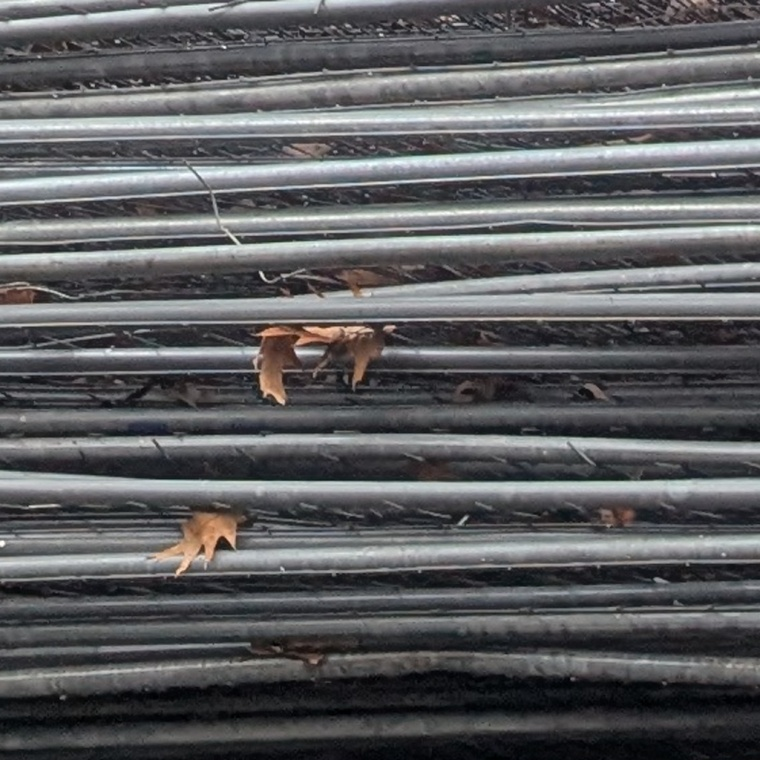
\includegraphics[width=\textwidth]{abbildungen/stufe_T1_hintergrund.jpg}
  \caption{T1 Hintergrund}
\end{subfigure}\hfill
\begin{subfigure}{0.315\textwidth}
  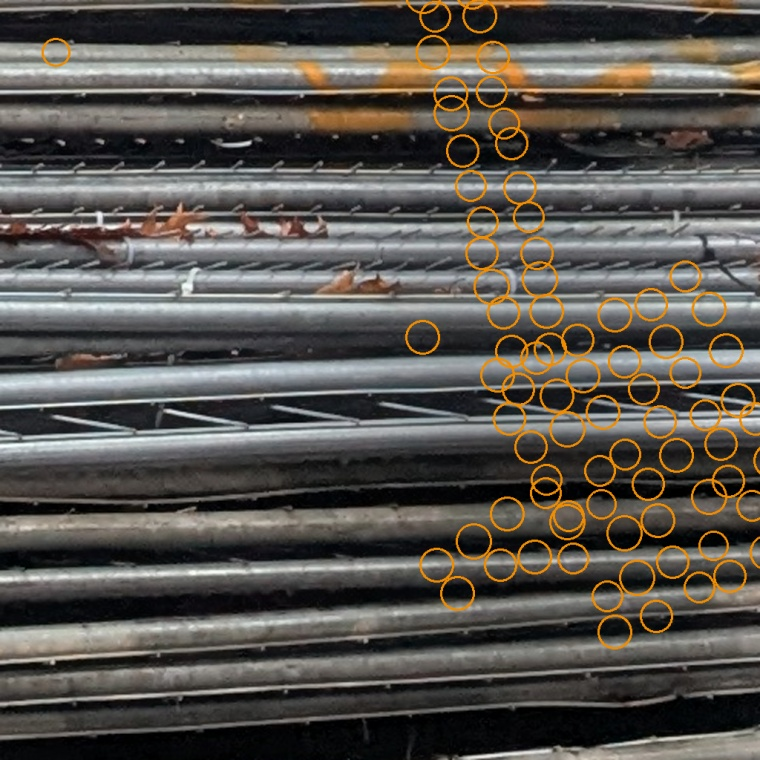
\includegraphics[width=\textwidth]{abbildungen/stufe_T4_layout.jpg}
  \caption{T4 Layout}
\end{subfigure}\hfill
\begin{subfigure}{0.315\textwidth}
  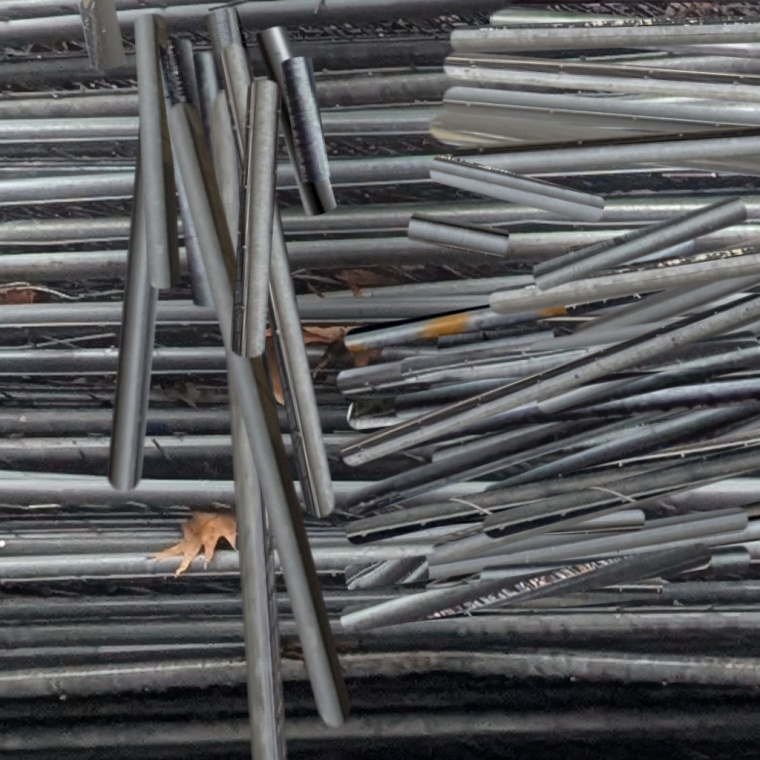
\includegraphics[width=\textwidth]{abbildungen/stufe_T5_schaft.jpg}
  \caption{T5 Rohrschaft}
\end{subfigure}

\vspace{4pt}
\begin{subfigure}{0.315\textwidth}
  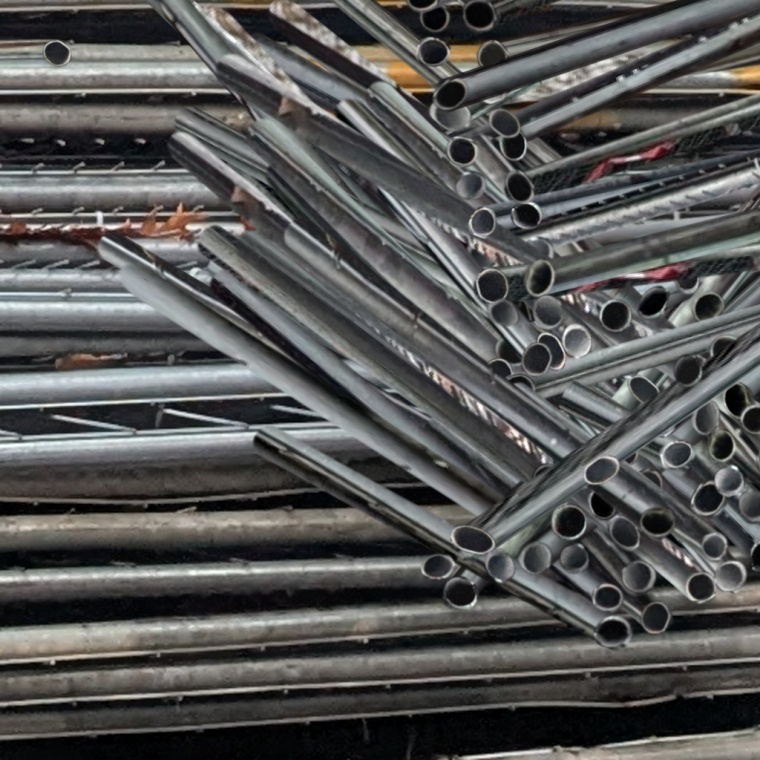
\includegraphics[width=\textwidth]{abbildungen/stufe_T2T3_instanzen.jpg}
  \caption{T2/T3 Instanzen}
\end{subfigure}\hfill
\begin{subfigure}{0.315\textwidth}
  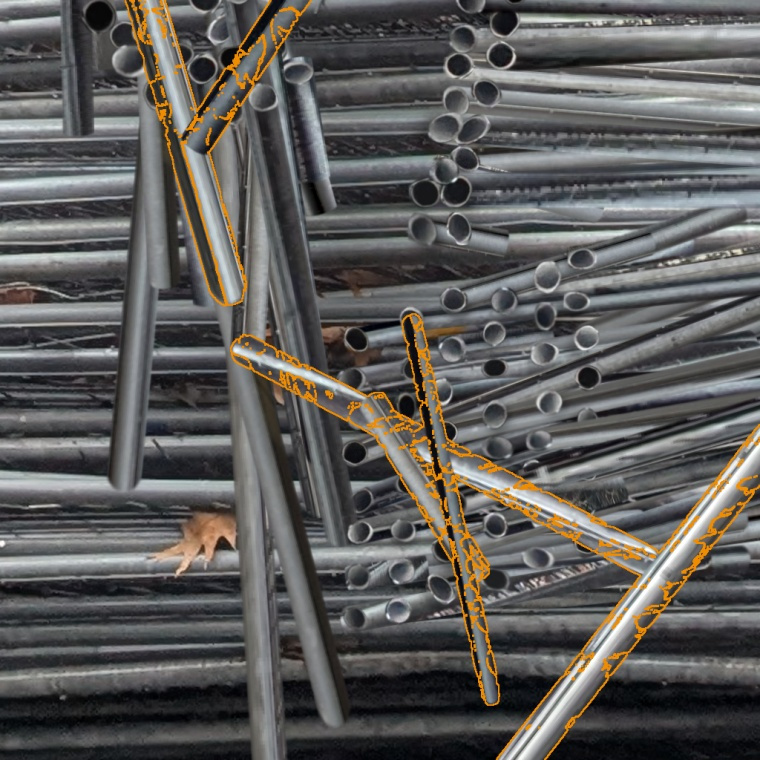
\includegraphics[width=\textwidth]{abbildungen/stufe_T6_okklusion.jpg}
  \caption{T6 Okklusion}
\end{subfigure}\hfill
\begin{subfigure}{0.315\textwidth}
  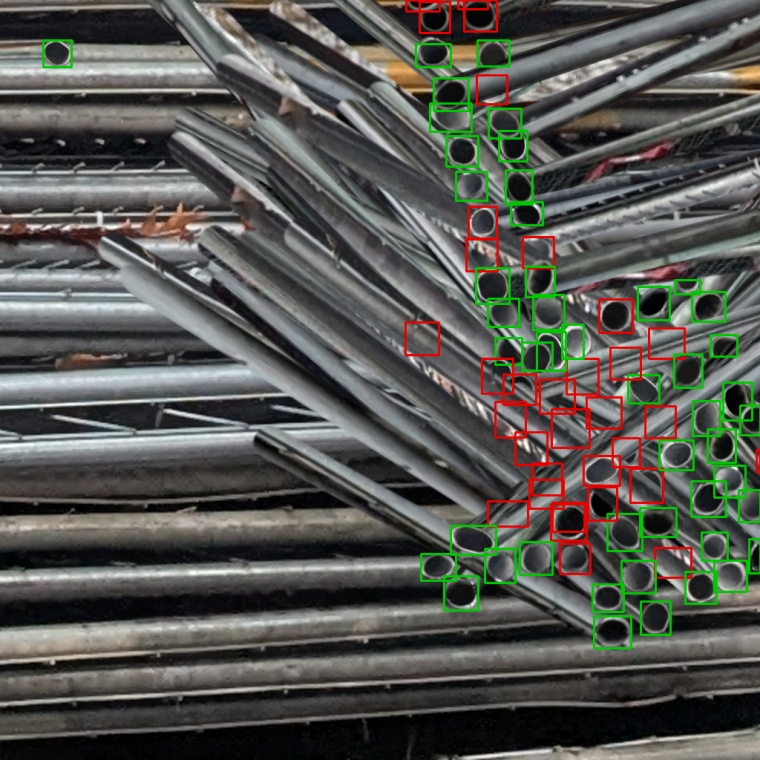
\includegraphics[width=\textwidth]{abbildungen/stufe_T7_sichtbarkeit.jpg}
  \caption{T7 Sichtbarkeit}
\end{subfigure}
% Instanzzahl auf 48 + 33 = 81 angeglichen (war 82). Falls im Bild
% tatsaechlich 82 Instanzen gerendert werden, ist eine davon vollstaendig
% verdeckt und erscheint in (f) weder gruen noch rot -- dann 82 behalten
% und in (f) ergaenzen: "eine Instanz ist vollstaendig verdeckt".
\caption[Aufbau eines synthetischen Bildes]{Aufbau eines synthetischen Bildes,
Stufe für Stufe am selben Bild. (a)~Der Clean Plate nach Zoom, Ausschnitt und
Spiegelung. (b)~Die gezogenen Objektzentren des Layoutmodells (orange), dazu
zwei abgedunkelte Mulden. (c)~Die Rohrschäfte in paralleler Richtung.
(d)~Die Stirnflächen mit Instanzgeometrie und Photometrie -- 81 Instanzen.
(e)~Die Ergänzungen der Okklusionsstufe, orange umrandet: sechs quer liegende
Stangen und Fremdkörper. (f)~Das Ergebnis der Sichtbarkeitsrechnung: grün die
48 vergebenen Labels, rot die 33 verworfenen Instanzen. Die Einzelstufen T2, T3, T8
und T9 sind in den Abbildungen~\ref{abb:stufendetail}
und~\ref{abb:stufenglobal} im Anhang vergrößert dargestellt. Zur Lesbarkeit ist
ein Bild am oberen Ende des Größenbereichs gewählt (Basisdurchmesser 44\px{}
statt des Medians von 23,5\px) und mit überdurchschnittlicher Verdeckung;
Abbildung~\ref{abb:synthbeispiele} zeigt typische Bilder. Erzeugt mit
\code{paper/tools/fig\_stufen.py}, Seed~302.}
\label{abb:stufen}
\end{figure}

\absatz{Maßstabskopplung.}\label{sec:modellentscheidungen} Der Zoomfaktor $z$ wird so gezogen, dass der
Basisdurchmesser im Zielbereich $[d_{\min}, d_{\max}]$ liegt:
\begin{equation}
z \sim \mathcal{U}\!\left[\max\!\left(z_{\min},\;
\tfrac{d_{\min}}{d_{\text{Rohr}}}\right),\;
\min\!\left(z_{\max},\;\tfrac{d_{\max}}{d_{\text{Rohr}}}\right)\right],
\qquad d_{\text{Basis}} = d_{\text{Rohr}} \cdot z .
\label{eq:zoom}
\end{equation}
Besetzt ist die Gleichung mit dem Zielbereich $[d_{\min}, d_{\max}] = [12, 44]$\px,
abgeleitet aus der an \code{val} und \code{test} gemessenen Spanne
12,2--35,8\px{} zuzüglich 25\,\% Reserve nach oben
(Tabelle~\ref{tab:statistik}), und mit der Maßstabsdeckelung
$[z_{\min}, z_{\max}] = [0{,}55;\,2{,}20]$, die \emph{gesetzt} ist und
verhindert, dass eine Clean Plate bis zur Unkenntlichkeit vergrößert oder so
weit verkleinert wird, dass ihre Rohrstruktur zur Textur zerfällt
(Tabelle~\ref{tab:parameter}). Der Rohrdurchmesser $d_{\text{Rohr}}$ ist keine
Konstante, sondern wird je Clean Plate über den Struktur-Tensor gemessen
(\code{src/occluders.py}, Abschnitt~\ref{sec:matting}). Objektgröße und
Hintergrundmaßstab sind damit \emph{nicht} unabhängig gezogen; das ist der Kern von Anforderung~A3.

Eine Einschränkung ist zu benennen: Die obere Klammer greift bei zwei der vier
Clean Plates und beschneidet dort den Zielbereich, sodass Basisdurchmesser über
39,6\px{} nur auf den beiden Clean Plates mit 20 und 21\px{} Rohrdurchmesser
entstehen. Objektgröße und Hintergrundwahl sind am oberen Ende des
Größenbereichs damit korreliert -- die Art von Kopplung also, die das
Leitprinzip dieses Kapitels vermeiden soll; die erzeugte
Größenverteilung endet entsprechend bei gut 40 statt 44\px{}
(Abschnitt~\ref{sec:datensatz}). Die untere Klammer greift dagegen nie. Für die
drei Fremdszenen ist Gleichung~\eqref{eq:zoom} mangels $d_{\text{Rohr}}$ nicht
definiert; dort werden Zoom und Objektgröße unabhängig gezogen
(Tabelle~\ref{tab:parameter}).

\absatz{Skalierung und Ovalisierung} werden in einem Schritt ausgeführt. Mit
Quelldurchmesser $d_{\text{src}}$, Zieldurchmesser $d$ und gezogenem
Achsverhältnis $\rho = s_y/s_x$ gilt $s_x = d/(d_{\text{src}}\sqrt{\rho})$ und
$s_y = d\sqrt{\rho}/d_{\text{src}}$, also $\sqrt{s_x s_y}\,d_{\text{src}} =
d$. Der geometrische Mittelwert bleibt damit erhalten; das ist notwendig,
damit die Ovalisierung die kalibrierte Größenverteilung nicht verschiebt, denn
die Realmessung verwendet mit $\sqrt{\text{Fläche}}$ genau dieses Maß. Die
\emph{Box} ändert sich dabei hingegen, und deren Seitenverhältnis ist die an
den Realdaten gemessene Größe. Zu beachten ist die Richtung: Bei kreisförmiger
Quelle ist das resultierende Seitenverhältnis $w/h$ der \emph{Kehrwert} von
$\rho$, ein oblates Objekt ($w/h > 1$) entsteht also aus $\rho < 1$.

\absatz{Farbangleich.} Ein \emph{partieller} Statistiktransfer im Stil von
\textcite{reinhard2001}: Mit Mittelwert und Streuung der Objektpixel
($\mu_i, \sigma_i$) und des lokalen Hintergrunds ($\mu_b, \sigma_b$) gilt je
Farbkanal
\begin{equation}
c' = \mu_i + k\,(c - \mu_i) + \alpha_\mu\,(\mu_b - \mu_i),
\quad
k = 1 + \alpha_\sigma\!\left(\operatorname{clip}\!\left(
\tfrac{\sigma_b}{\sigma_i},\, r_{\min},\, r_{\max}\right) - 1\right)
\label{eq:harmonize}
\end{equation}
Die freien Größen sind Sollwerte aus \code{src/generate.py} und in
Tabelle~\ref{tab:parameter} als \emph{gesetzt} ausgewiesen: Die Angleichstärken
werden je Instanz als $\alpha_\mu \sim \mathcal{U}[0{,}10;\,0{,}45]$ und
$\alpha_\sigma \sim \mathcal{U}[0;\,0{,}35]$ gezogen, das Streuungsverhältnis
wird auf $[r_{\min}, r_{\max}] = [0{,}6;\,1{,}6]$ begrenzt, damit eine besonders
glatte oder besonders unruhige Einfügestelle den Objektkontrast nicht
umkehrt. Für
$\alpha_\mu = \alpha_\sigma = 1$ entstünde der vollständige Reinhard-Transfer;
er bleibt unangewendet, weil er den intrinsischen Albedo-Unterschied zwischen
Bohrung und Kranz einebnete (Abbildung~\ref{abb:farbangleich}). Modelliert wird ausschließlich die
Beleuchtungs- und Weißabgleichdifferenz, nicht die Objektfarbe. Begründet ist
damit die \emph{Richtung}, nicht der Betrag: Die vier Grenzen sind gesetzt und
stehen in Tabelle~\ref{tab:parameter} als Annahme.

\begin{figure}[htbp]
\centering
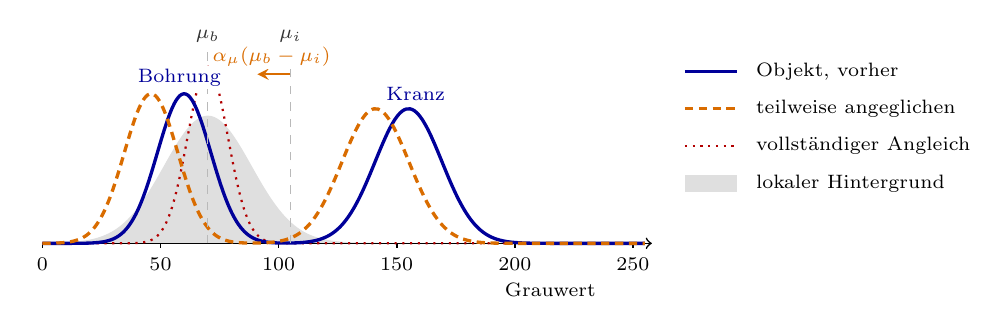
\begin{tikzpicture}[x=0.030cm,y=1.9cm]
  \draw[gray!25,fill=gray!25,smooth]
    plot[domain=0:255,samples=110] (\x, {0.85*exp(-((\x-70)/26)^2)})
    -- (255,0) -- (0,0) -- cycle;
  \draw[->,semithick] (0,0) -- (258,0);
  \node[font=\scriptsize,anchor=north] at (215,-0.20) {Grauwert};
  \foreach \g in {0,50,100,150,200,250}
    \draw[semithick] (\g,0) -- (\g,-0.030) node[below,font=\scriptsize] {\g};
  \draw[red!70!black,thick,dotted,smooth]
    plot[domain=0:255,samples=150] (\x, {1.18*exp(-((\x-70)/12)^2)});
  \draw[very thick,blue!60!black,smooth]
    plot[domain=0:255,samples=150]
    (\x, {exp(-((\x-60)/16)^2) + 0.9*exp(-((\x-155)/20)^2)});
  \draw[very thick,orange!85!black,densely dashed,smooth]
    plot[domain=0:255,samples=150]
    (\x, {exp(-((\x-46)/16)^2) + 0.9*exp(-((\x-141)/20)^2)});
  \draw[dashed,gray!55] (70,0) -- (70,1.34);
  \node[font=\scriptsize,gray!40!black,anchor=south,fill=white,inner sep=1pt]
       at (70,1.32) {$\mu_b$};
  \draw[dashed,gray!55] (105,0) -- (105,1.34);
  \node[font=\scriptsize,gray!40!black,anchor=south,fill=white,inner sep=1pt]
       at (105,1.32) {$\mu_i$};
  \draw[->,>=stealth,orange!85!black,thick] (105,1.13) -- (91,1.13);
  \node[font=\scriptsize,orange!85!black,anchor=south,inner sep=1pt,
        fill=white] at (97,1.16) {$\alpha_\mu(\mu_b - \mu_i)$};
  \node[font=\scriptsize,blue!60!black,anchor=south,fill=white,inner sep=1pt]
       at (58,1.03) {Bohrung};
  \node[font=\scriptsize,blue!60!black,anchor=south,fill=white,inner sep=1pt]
       at (158,0.93) {Kranz};
  \begin{scope}[shift={(272,0)}]
    \draw[very thick,blue!60!black] (0,1.15) -- (22,1.15);
    \node[font=\scriptsize,anchor=west] at (26,1.15) {Objekt, vorher};
    \draw[very thick,orange!85!black,densely dashed] (0,0.90) -- (22,0.90);
    \node[font=\scriptsize,anchor=west] at (26,0.90) {teilweise angeglichen};
    \draw[thick,red!70!black,dotted] (0,0.65) -- (22,0.65);
    \node[font=\scriptsize,anchor=west] at (26,0.65) {vollständiger Angleich};
    \fill[gray!25] (0,0.34) rectangle (22,0.46);
    \node[font=\scriptsize,anchor=west] at (26,0.40) {lokaler Hintergrund};
  \end{scope}
\end{tikzpicture}
\caption[Partieller Farbangleich]{Partieller Farbangleich nach
Gleichung~\eqref{eq:harmonize}. Die Grauwertverteilung des Objekts ist
zweigipfelig: dunkle Bohrung und heller Kranz. Der Angleich verschiebt sie um
$\alpha_\mu(\mu_b - \mu_i)$ in Richtung des lokalen Hintergrunds, hält die
beiden Gipfel aber auseinander. Ein vollständiger Angleich (gepunktet) zöge sie
auf die Hintergrundverteilung zusammen und zerstörte damit den
Albedo-Unterschied, der das Objekt überhaupt erkennbar macht.}
\label{abb:farbangleich}
\end{figure}

\absatz{Rauschschätzung.} Das lokale Rauschniveau wird als Streuung des
Hochpassrests $\hat{\sigma} = \operatorname{std}(g -
\operatorname{median}_{3\times3}(g))$ geschätzt
\parencite[vgl.][]{immerkaer1996} -- Medianfilter als Tiefpass, weil er Kanten
weniger verschmiert -- und als $\sigma_{\text{Rausch}} = \max(0{,}5,\,
\hat{\sigma}\cdot\mathcal{U}[0{,}5;\,1{,}25])$ eingefügt. Ohne
Normierungsfaktor überschätzt $\hat\sigma$ systematisch und geht deshalb nur
als \emph{relatives} Maß ein. Diese Grenze wie auch die Klammerung von
$\sigma_b/\sigma_i$ auf $[0{,}6;\,1{,}6]$ sind Absicherungen gegen entartete
Schätzwerte bei uniformem Hintergrundfleck oder rauschfreiem Ausschnitt; sie
behaupten nichts über die Zieldomäne und zählen nicht zu den in
Tabelle~\ref{tab:parameter} bilanzierten Parameterwerten.

\absatz{Layoutmodell.} Pro Cluster mit Basisdurchmesser $d_0$ liegen die
Objektzentren auf einer gescherten, verrauschten Gitterpackung
\begin{equation}
p_{ij} = i\,g_1\,\mathbf{e}_1 + j\,g_2\,\mathbf{e}_2 + \mathbf{c}
+ \boldsymbol{\epsilon}_{ij},
\qquad \boldsymbol{\epsilon}_{ij} \sim \mathcal{N}\!\big(\mathbf{0},
\sigma_G^2\, \mathbf{I}\big),
\label{eq:layout}
\end{equation}
mit Gitterabständen $g_1 \in [g_1^-, g_1^+]\,d_0$, $g_2 \in [g_2^-, g_2^+]\,d_0$,
einem eingeschlossenen Winkel aus $[\gamma_{\min}, \gamma_{\max}]$ und der
Rauschstärke $\sigma_G = c_\sigma\,d_0$. Eingesetzt werden
$[g_1^-, g_1^+] = [0{,}98;\,1{,}60]$, $[g_2^-, g_2^+] = [0{,}98;\,1{,}85]$,
$[\gamma_{\min}, \gamma_{\max}] = [55^\circ;\,125^\circ]$ und
$c_\sigma = 0{,}17$. Diese vier Werte sind nicht gesetzt, sondern an der
erzeugten Statistik gegen die Realmessung kalibriert: die Obergrenzen der
Gitterabstände an Median und p90 des NN-Abstands, der Winkelbereich am
Histogramm der Nachbarrichtungen, $c_\sigma$ an p10 und Berührungsquote
(Tabelle~\ref{tab:kalibrierung}; Belegart je Wert in
Tabelle~\ref{tab:parameter}, Block T4). Ohne den Rauschterm
$\boldsymbol{\epsilon}_{ij}$ entstünden sichtbar künstliche Reihen; er
verschiebt jede Lage im Mittel um
$\mathbb{E}\lVert\boldsymbol{\epsilon}\rVert = c_\sigma\,d_0\sqrt{\pi/2}
\approx 0{,}21\,d_0$. Die Untergrenze der Gitterabstände ist physikalisch -- Rohrzentren können sich nicht durchdringen --, die zwei Prozent Spiel tragen der
Messkonvention Rechnung: $d_0$ ist über die \emph{modale} Box definiert, die bei
verdeckten Objekten kleiner ausfällt als das Rohr selbst, weshalb schon der
gemessene NN-Abstand mit p10 $=0{,}86$ (\code{val}) bzw.\ $0{,}78\,\Oe$
(\code{test}) unter einem Durchmesser liegt. Die Bereiche der Einzelparameter
stehen in Tabelle~\ref{tab:parameter}; sie sind nicht gemessen, sondern iterativ
so eingestellt, dass die erzeugte Anordnung die in
Tabelle~\ref{tab:kalibrierung} gegenübergestellten Kenngrößen der Realbilder
trifft. Das Clusterzentrum $\mathbf{c}$ darf außerhalb der Leinwand liegen,
sodass angeschnittene Objekte am Bildrand entstehen (Befund~9).


\absatz{Sichtbarkeitsrechnung und Labels.}\label{sec:sichtbarkeit} Labels dürfen in einem Copy-Paste-Generator nicht ungeprüft vergeben werden.
Für \emph{jede} Instanz wird die Sichtbarkeit daher exakt berechnet. Grundlage ist die
Alpha-Kompositionsregel von \textcite{porter1984}: Wird Instanz $i$ von allen
später gezeichneten Schichten $j$ überlagert, so ist ihr sichtbarer Anteil
\begin{equation}
\alpha_i^{\text{sichtbar}} = \alpha_i \prod_{j > i} \big(1 - \alpha_j\big),
\qquad
v_i = \frac{\textstyle\sum \alpha_i^{\text{sichtbar}}}{\textstyle\sum \alpha_i},
\label{eq:sichtbarkeit}
\end{equation}
wobei das Produkt über \emph{alle} später gezeichneten Schichten läuft, einschließlich anderer Profile, Rohrschäfte und Fremdkörper.

Daraus folgen die Verwerfungsregeln, dieselben, nach denen \code{val} und
\code{test} annotiert wurden (Anforderung~A1). Ein Label wird verworfen, wenn
die Sichtbarkeit unter 30\,\% liegt -- \emph{kein} Label macht dieselbe
Bildstelle zum korrekten harten Negativ --, wenn weniger als 15\,\% der Fläche
im Bild liegen, oder wenn die sichtbare Box unter 5\px{} fällt. Vergeben wird
stets die \emph{modale} Box, also der sichtbare Umriss.

Verworfen werden insgesamt 36\,716 der 173\,100 gerenderten Instanzen
(21,2\,\%), der weitaus größte Teil davon durch die Sichtbarkeitsregel. Die
Aufschlüsselung nach Ursachen steht im Erzeugungsbericht
(Abschnitt~\ref{sec:anhangbericht}). Diese Instanzen sind kein
Verlust, sondern der Ertrag der Stufe: Sie markieren jene Bildstellen, an
denen ein naiver Generator ein falsches Label gesetzt hätte.

\section{Der erzeugte Datensatz}
\label{sec:datensatz}

Alle Zahlen dieses Abschnitts stammen aus dem Erzeugungsbericht
\code{generation\_report.json}, den der Generator neben jeden Datensatz
schreibt; Abschnitt~\ref{sec:anhangbericht} listet ihn vollständig auf.
Es entstehen 6000 Bilder zu $1024\times1024$ Pixeln, davon 583 Negativbilder
(9,7\,\%), mit 136\,384 gelabelten Objekten (22,7 je Bild über alle 6000, also
25,2 je Positivbild) aus 173\,100 gerenderten Instanzen. Die mittlere
Sichtbarkeit der gelabelten Objekte beträgt 90,0\,\%, 30,1\,\% von ihnen sind
teilverdeckt.

Der wichtigste Qualitätsnachweis ist nicht der optische Eindruck, sondern der
Vergleich der erzeugten mit der gemessenen Statistik. Tabelle~\ref{tab:kalibrierung}
stellt beide gegenüber und enthält damit auch die Größen- und
Seitenverhältnisverteilung des erzeugten Datensatzes.

\begin{table}[htbp]
\centering
\caption[Kalibrierung gegen die Realmessung]{Kalibrierung des Layoutmodells
gegen die Realmessung ($n = 187$). Alle Abstände in Objektdurchmessern; die
synthetischen Werte sind über 1500 erzeugte Bilder mit 34\,027 Labeln gemessen.}
\label{tab:kalibrierung}
\footnotesize
% Die Durchmesserzeile stand im Kopf auf p95, trug real aber p90-Werte
% (vgl. tab:statistik) und synthetisch einen p95-Wert. Da fuer die realen
% Splits kein p95 und fuer die synthetische Verteilung kein p90 vorliegt,
% ist die Zeile jetzt auf p05 und Median beschraenkt; das obere Ende wird
% im Text mit dem p95 von 39,9 px diskutiert. Liegen beide Perzentile
% vor, kann die dritte Spalte wieder ergaenzt werden.
% Die Seitenverhaeltniszeile ist konsistent (durchgaengig p10/Median/p90);
% die Abweichung zum frueheren Textwert 1,40 kam allein vom kleineren
% Stichprobenumfang und ist in der Bildunterschrift erklaert.
\begin{tabular}{@{}lccc@{}}
\toprule
\textbf{Kenngröße} & \textbf{real \code{val}} & \textbf{real \code{test}} &
\textbf{synthetisch (Ist)} \\
\midrule
NN-Abstand p10 / Median / p90 & 0,86 / 1,11 / 1,78 &
0,78 / 1,26 / 2,72 & \textbf{0,84 / 1,17 / 1,90} \\
NN näher als $1{,}2\,\Oe$ & 60,2\,\% & 44,9\,\% & \textbf{53,5\,\%} \\
Nachbarn innerhalb $5\,\Oe$ (Median) & 10 & 10 & \textbf{13} \\
Größenverhältnis zum NN (Median) & 1,05 & 1,07 & \textbf{1,10} \\
Objektdurchmesser p05 / Median (px) & 19,1 / 26,8 &
12,2 / 17,0 & \textbf{12,0 / 23,5} \\
Seitenverhältnis p10 / Median / p90 & 0,97 / 1,09 / 1,40 &
0,82 / 1,08 / 1,22 & \textbf{0,78 / 1,00 / 1,33} \\
\bottomrule
\end{tabular}
\end{table}

Die synthetische Verteilung liegt bei fast allen Kenngrößen zwischen oder nahe
bei den beiden realen Messungen. Zwei systematische Abweichungen bleiben. Die
erste ist die Nachbarzahl: Die synthetischen Cluster sind dichter (13 statt 10
Nachbarn innerhalb $5\,\Oe$, im Maximum 61 statt 20). Das ist bewusst so
belassen: Eine höhere Dichte im Training ist eine Robustheitsreserve, weil sie
den Detektor auf schwierigere Szenen vorbereitet als die, die er zur
Inferenzzeit vorfindet; die umgekehrte Abweichung wäre problematisch. Die
zweite betrifft die Objektgröße: Der Generator soll 12--44\px{} abdecken,
erreicht am oberen Ende aber nur gut 40\px{} (p95 der erzeugten Verteilung:
40,4\px); das ist eine Folge der Zoomdeckelung nach Gleichung~\eqref{eq:zoom}.
Am unteren Ende enthält \code{test} vier Objekte unterhalb von 12\px{}
(kleinstes 6,4\px). Diese Lücke schließt erst die Trainingsskalierung, die die
Untergrenze nach Gleichung~\eqref{eq:effgroesse} auf $d_{\min}\,(1-a) =
7{,}2$\px{} zieht (Abschnitt~\ref{sec:trainparam}); die vier kleinsten Objekte
in \code{test} liegen auch dann noch am unteren Rand der Trainingsverteilung.

\section{Nachweis der Anforderungen}
\label{sec:nachweis}

\begin{table}[htbp]
\centering
\caption[Nachweis der Anforderungen]{Umsetzung der sechs Anforderungen aus
Abschnitt~\ref{sec:anforderungen}. Die letzte Spalte nennt, wo die Wirksamkeit
der Maßnahme experimentell geprüft wird.}
\label{tab:nachweis}
\footnotesize
\begin{tabularx}{\textwidth}{@{}lXl@{}}
\toprule
& \textbf{Umsetzung} & \textbf{geprüft} \\
\midrule
A1 & Box aus transformierter Alphamaske; \code{degrees}, \code{shear},
     \code{perspective} $=0$; Verwerfungsregeln wie bei der Handannotation
   & \ref{sec:boxversatz} \\
A2 & Leinwand $=$ Trainingsauflösung; 12--44\px, faktisch bis 40\px{}
     (Gl.~\eqref{eq:zoom}) & -- \\
A3 & Maßstabskopplung, Schaft bei 88\,\% der Instanzen, parallele
     Schaftrichtung, Tiefenmodell 75/25, volle Rotation & -- \\
A4 & S1 Alphamaske und Kantenweichzeichnung, S2 partieller Farbangleich,
     S3 flächentreue Skalierung und Unschärfeangleich, S4 Rauschangleich,
     S5 JPEG-Requantisierung, S6 Schlagschatten und physikalische Verdeckung;
     photographische Okkluder-Bibliothek gegen S2--S4
   & \ref{sec:ablationB} \newline (Okkluder), \newline \ref{sec:ablationC}
     \newline (S1--S5 als \newline Bündel) \\
A5 & Tabelle~\ref{tab:parameter}: Sollbereich und gemessener Ist-Anteil je
     Transformation; Erzeugungsbericht je Datensatz & -- \\
A6 & Belegart je Parameterwert; die beiden numerischen Absicherungen
     ausdrücklich ausgenommen & -- \\
\bottomrule
\end{tabularx}
\end{table}

Tabelle~\ref{tab:nachweis} stellt die Umsetzung der sechs Anforderungen
zusammen. Sie sind damit \emph{formal} erfüllt; die Erfüllung einer
Entwurfsanforderung ist aber kein empirischer Nachweis, wie ihre letzte Spalte
zeigt. Wie viel von den 44 Parameterwerten der 37 Transformationen tatsächlich
belegt ist, bilanziert Abschnitt~\ref{sec:tragend}.